\section{Architecture}
\label{Arc}
\subsection{SDN Preliminaries}
Before introducing our SDN system architecture, we first present some general terms including three planes and two interfaces in SDN system \cite{kreutz2015software}.

A data plane is the part of a network that carries user traffic and basic sensing functions. And a control plane is the part of a network that carries signaling traffic and is responsible for routing. The top layer of SDN system is management plane which includes the software services, such as simple network management protocol (SNMP). It used to remotely monitor and configure the control functionality. The user implement their applications on it.

Southbound Interface (SI) is the instruction set of the forwarding devices is defined by the southbound API, which is part of the southbound interface. Furthermore, the SI also defines the communication protocol between data plane and control plane elements. This protocol formalizes the way the control and data plane elements interact. Northbound Interface (NI) is the middleware on control plane can offer an API to application developers.

\subsection{Overview of {\sdn}}
The architecture of {\sdn} is shown in Fig. \ref{Architecture}. 
The system is divided into three layers and two interface abstraction, the southbound interface connect data plane and control plane, and the nouthbound interface connect control plane and management plane. In our system, the data plane runs on sensor nodes. The control plane and management plane runs on more powerful UAVs.
\begin{figure}[htbp]
	\centering
	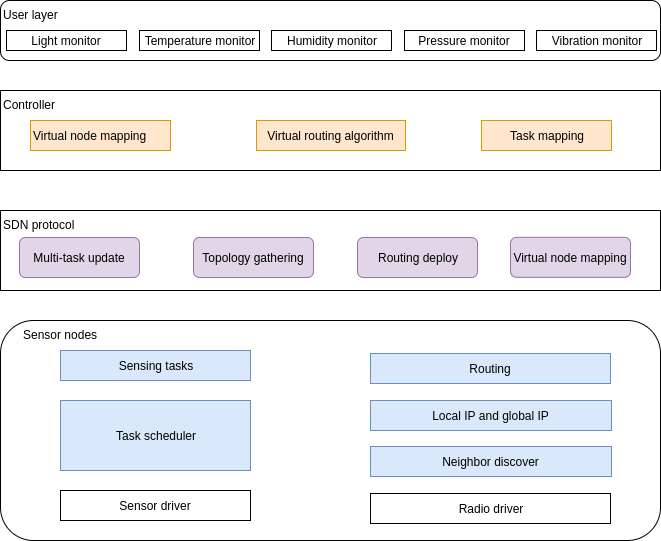
\includegraphics[width=3.5in]{./Figure/Architecture}
	\caption{Architecture of the system.}
	\label{Architecture}
\end{figure}

To build software defined network system in WSN and achieve low 
energy consumption and high performance, the SDN controller ought to  
configure data plane within as less hops as possible.  
In {\sdn}, we choose UAV as a mobile SDN controller,  
which communicates with sensor nodes by on-hop communication.
It significantly reduces the energy consumption of nodes in {\sdn}. 
To achieve high performance, the UAV controller carries
a powerful airborne computer which has ability to run 
some intelligent applications in real-time.

\subsection{SDN Planes of {\sdn}}
The \textbf{data plane} runs on sensor nodes contains four components, including neighbor discovery, routing mapping, radio duty cycle control and data sampling. We abstract the function running on sensor nodes to southbound interface. Our clearly abstraction of data plane functions make the SDN system work efficiently.

In the \textbf{control plane} of {\sdn}, in order to make our system easy to use, we implement a database on the UAV and design interfaces for data plane and SDN applications. The control plane connected data plane and management plane. The database maintain the topology gathered from the data plane, route table inputed form applications, and sensor task schedule table form management application.

On \textbf{management plane}, user can run tons of applications base on our well-defined southbound APIs, such as routing algorithms, network diagnose, sensor task 
scheduler, etc. Our system is capable to run application together. We design and implement five applications on {\sdn}. The detail design of our applications is described in section \ref{App}. 

As shown in Fig. \ref{Architecture}, both the upward data flow and downward SDN commands transfer smoothly by using our well defined interface. Take the topology gathering as an example, the control plane receives nodes neighbor table through southbound interface, it saves the topology in database. After UAV gathered all nodes' neighbor table, the topology management module arrange nodes neighbor table in database and get the whole network topology for management applications such as routing protocol application to read. Another example is sensor's task deployment, the task scheduler application outputs the task schedule table to control plane. Then the task management module save it to database. When UAVs is near sensor nodes, it get the task table for specific nodes from database. 

Different from wired network, the data plane of WSN not only runs
data forwarding function, but also executes data sampling function. 
For example,  sensor nodes execute neighbor discovery process for getting topology, 
data sampling process for getting data from environment and data forwarding process
for data gathering. {\sdn} is an easy-to-use system that we design and implement a lot of 
interfaces for users. The detail implementation of our system is introduced in section \ref{Imp}.
\subsection{Nouthbound Data Structures}

As shown in Fig \ref{downstream} and Fig \ref{upstream}, the \textbf{nouthbound data structure} including downstream and upstream structure fully considered the difference between wired networks and wireless sensor networks, the data structure not only contains routing  related data, but also has sensor task control tables.

\begin{figure}[htbp]
	\centering
	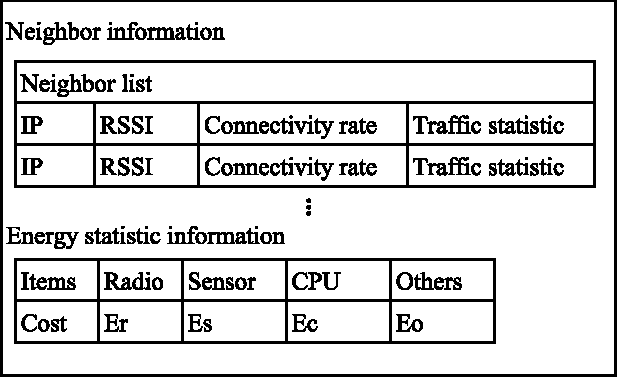
\includegraphics[width=.8\columnwidth]{Figure/upstream}
	\caption{Upstream data structure}
	\label{upstream}
\end{figure}

The upstream data is input for routing protocol, it including neighbor information collected by node neighbor discovery. 
When node runs neighbor, it also records the received signal strength indicator (RSSI) of every neighbor nodes. To keep neighbor table freshness, 
node will execute neighbor discovery periodically base on user defined interval.
Moreover, node also records some statistic information including the data traffic and energy consumption for control plane to optimize and diagnose the network.

\begin{figure}[htbp]
	\centering
	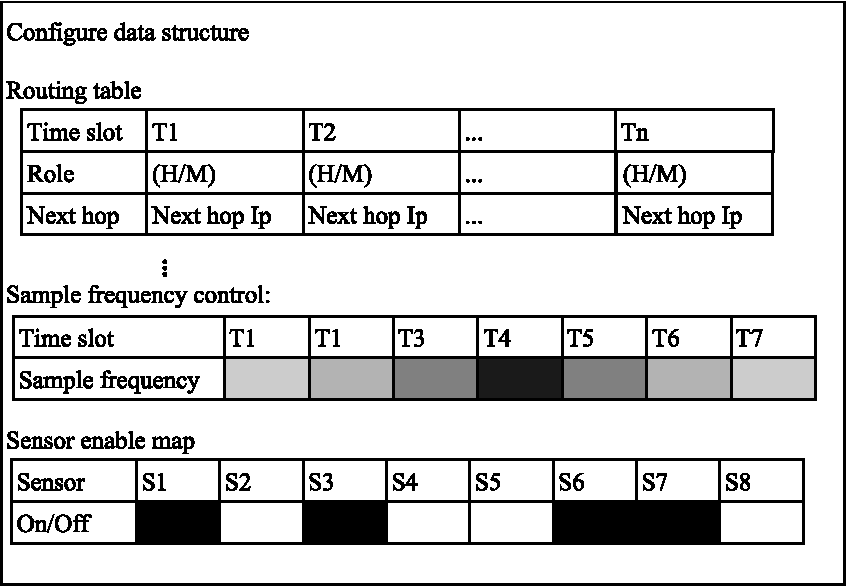
\includegraphics[width=.8\columnwidth]{Figure/downstream}
	\caption{Downstream data structure}
	\label{downstream}
\end{figure}

The downstream data is the configuration data that control plane send to data plane. In wireless sensor networks, 
the configuration data including routing table, sensor sampling control table and sensor task map, the specific explaination of data structure will discuss in section \ref{App}.

\subsection{Southbound Interface}
The Table \ref{API} shows our southbound interface for user write applications. By using our SDN Southbound Interface, users can easily write 
a variety of applications, such as routing protocol, sensor task scheduler, network diagnose, algorithm evaluator, etc.
\begin{table*}[!b]
	\caption{SDN Southbound Interface}
	\label{API}
	\centering
	\scalebox{0.9}{
	\begin{tabular}{|l|l|}
		\hline
		\makecell[tc]{\textbf{Structure \&\& Function}} & \makecell[tc]{\textbf{Description}} \\
		\hline
		\multicolumn{2}{|c|}{\textbf{Sensor Control Interface}}\\
		\hline 
		\hline
		struct node & Sensor node structure\\
		\hline
		struct nodeset & A set of sensor nodes \\
		\hline
		struct neighbor\_list & Neighbor infomation \\
		\hline
		struct energy\_item & Energy statistic information \\
		\hline
		struct rout\_table & Route table \\
		\hline
		struct duty\_cycle\_table & Duty cycle control table \\
		\hline
		struct sensor\_enable\_table & All the nodes's states. Node state: \{on,off\} \\
		\hline
		switch\_node(node,state) & Turn on or turn off the node \\
		\hline
		get\_node\_info(node) & Get node's information, including  node's position, duty cycle, power, etc.\\
		\hline
		set\_node\_attr(node,attrTag,value) & Set node attribute, including  duty cycle, radio strength, etc. \\
		\hline
		get\_neighborlist(node) & Get the neighbor list of a node \\
		\hline
		\multicolumn{2}{|c|}{\textbf{UAV Application Interface}}\\
		\hline
		\multicolumn{2}{|c|}{\textbf{Routing}}\\
		\hline 
		\hline
		get\_topology() & Get the topology of the network\\
		\hline
		get\_rout\_table(node) & Get the route table of a node \\
		\hline
		set\_route(node) & Set the route of a node \\
		\hline
		\multicolumn{2}{|c|}{\textbf{AI Node selection}}\\
		\hline
		\hline
		nodeset simple\_selection(nodeset) & Select sensor set by location information\\
		\hline
		nodeset SRSSS\_selection(dataset) & Select sensor set by AI algorithm based on sensing data\\
		\hline
		\multicolumn{2}{|c|}{\textbf{AI Energy Prediction}}\\
		\hline
		\hline
		model\_selsct(modeltype) & Select an AI model\\
		\hline
		model.train(dataset,ratio) & Train an AI model with learning ratio on the data set\\
		\hline
		model.test(dataset) & Test the AI model on the data set\\
		\hline
		model.predict(node) & Do the energy prediction for a node \\
		\hline
		\multicolumn{2}{|c|}{\textbf{Multi-tasks}}\\
		\hline
		\hline
		create\_scheduler() & Create a task scheduler \\
		\hline
		scheduler.create\_buffer() & Create a task buffer \\
		\hline
		scheduler.task\_buffer\_add(task,nodeset) & Add a new task to task buffer \\
		\hline
		scheduler.task\_buffer\_remove(task) & Remove a new task to task buffer \\
		\hline
		scheduler.task\_buffer\_update(task,nodeset) & Update a task to task buffer with a new nodeset \\
		\hline
		scheduler.task\_update() & Schedule the added or removed tasks in the buffer\\
		\hline
		\multicolumn{2}{|c|}{\textbf{Diagnosis}}\\
		\hline
		\hline
		detect() & Detect problematic region with probes \\
		\hline
		get\_topical\_topology(nodeset) & Construct topical topology\\
		\hline
		diagnose\_network(topology,nodeset) & Diagnose the failure nodes or lossy links\\
		\hline
	\end{tabular}
	}
\end{table*}

We demonstrate two application code using our southbound interface and write the code in in Section \ref{subsectionrouting} and Section \ref{subsectionmultitask}.

